\section{Testing and Evaluation Methodologies}
\label{sec:testing_and_evaluation_methodologies}

\subsection{Proposed Methods for Testing}
\label{sec:proposed_methods_for_testing}

\subsubsection{Unit}\label{ss:unit}
For each individual software component (class, method, etc.) developed in the project, an associated unit-test will be deployed to verify its correctness. The Catch2 testing framework~\cite{catch2} appears to be an ideal means to allow this, with header-only requirements on the C++ layer, and is available under the Boost Software License.
%---------------------------------------------------------------------------------

\subsubsection{Integration}\label{ss:integration}
Like unit testing, we can again rely on the Catch2 framework to implement integration tests using a well-defined set of examples for each component of the Intel-QNLP suite. The use of continuous integration (CI) framework can be used to routinely examine these tests.

%---------------------------------------------------------------------------------

\subsubsection{Regression}\label{ss:regression}
As with Section~\ref{ss:integration}, we can use CI frameworks to perform periodic tests of those outlined for the previous levels of granularity in Unit and Integration tests, but also consider additional metrics such as:
\begin{itemize}
    \item Vectorisation and threading
    \item Strong and weak scaling
    \item Memory occupancy
    \item Compute and memory intensity using roofline models
    \item MPI load-balancing
    \item Additional compilation options (inter-procedural/link-time optimisation, compiler optimisation levels, fast-math, etc.) 
\end{itemize}

%---------------------------------------------------------------------------------

\subsection{Proposed Methods for Evaluation}
\label{sec:proposed_methods_for_evaluation}

\subsubsection{Acceptance}\label{ss:acceptance}
This final level of testing and evaluation will be used to determine overall correctness of the routines with a set of well-known results for the suite. We can use a manually-defined model, and compare the results to the computed data in an automated manner, making use of the CI testing methods as proposed by the Section~\ref{ss:integration}. Additionally, we may use classical NLP methods to compare results with the implemented DisCo model, such as discussed below.

%---------------------------------------------------------------------------------

\paragraph{spaCy:}
spaCy~\cite{spacy2} provides an industry-backed framework for natural language processing, which includes semantic comparison, and diagrammatic dependency visualisation. For the diagrammatic structure proposed by Zeng et al.~\cite[Example 5.3]{Zeng_Coecke_2016}, the authors derive a graph for computing the meaning of a sentence using the proposed DisCo framework. While subtle differences exist, a similar graphical style can be obtained through use of the spaCy \textit{displaCy} module. Figure \ref{fig:spacy_vs_disco} shows a comparison between both formats, wherein $(a)$ is derived manually using the model proposed by Zeng et al., and $(b)$ can be automatically derived using spaCy, both defined for the sentence ``\textit{John saw Mary read a book.}''. This provides us with a promising candidate for comparative analysis of structure for our proposed model and implementation. Additionally, spaCy provides semantic similarity comparison based on use of word-vectors, provides us with a direct means to evaluate sentence similarity using classical NLP methods. 

%---------------------------------------------------------------------------------

\paragraph{SEMILAR:}
SEMILAR~\cite{semilar_2013} is a Java tool-kit for performing semantic sentence similarity analysis on text corpora. We have not currently investigated its use for this task, but leave it as a potential means to generate comparative data as a future task.

\begin{figure}[H]
    \centering
    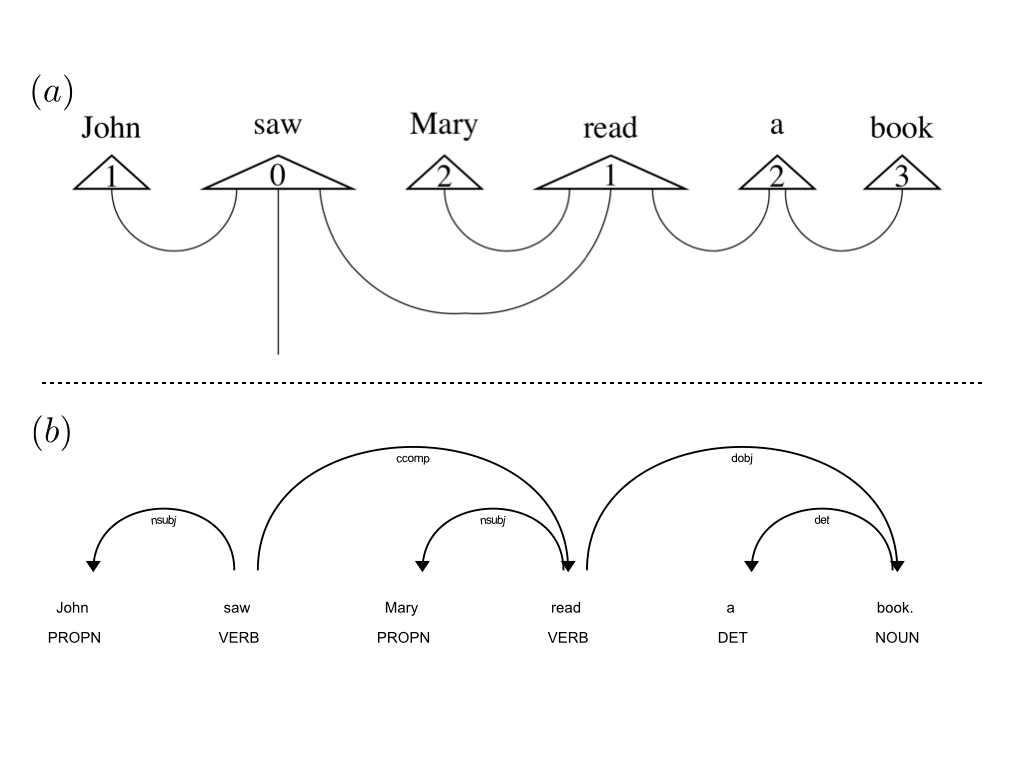
\includegraphics[width=0.85\linewidth,trim=0 20px 0 20px]{D1_1/Images/spacy_vs_CSC.png}
    \caption[DisCo model versus spaCy sentence analysis.]{Sentence parsing structure for $(a)$ the DisCo model, and $(b)$ that from the classical NLP package spaCy.}
    \label{fig:spacy_vs_disco}
\end{figure}

%---------------------------------------------------------------------------------
